Verwendete technische Konzepte, sowie benötigte Software werden in diesem Kapitel genauer beschrieben.

\section{Altium}\label{sec:3.1}
\enquote{Altium Designer} ist eine Software zum Entwickeln und Designen von elektronischen Leiterplatten (engl. PCB). In unserem Fall wurde die Version 13.3 verwendet. 
\begin{figure} [H]
	\centering
	
\includegraphics[width=1\textwidth]{img/ad_logo.png}
	\caption{Logo von \enquote{Altium Designer} (\url{http://www.altium.com/resources/images/media-release/ad_logo.png})}
	\label{fig:3.1.1}
\end{figure}

Für jedes neues \enquote{PCB}-Projekt muss eine \enquote{Schematic}-Datei und eine \enquote{PCB}-Datei angelegt werden.


%http://www.altium.com/resources/images/media-release/ad_logo.png

\subsection{Einstellungen für die PCB-Entwicklung}
%% Altium und Einstellungserklärung + Wichtige Layout-Faktoren
%Beim designen des Leiterplattenlayouts wurden die allgemeinen Altium-Einstellungen vorgenommen und auf die zu berücksichtigenden Layoutpunkte geachtet.
Beim \enquote{Layouten} der Schaltung in \enquote{Altium Designer} mussten einige wichtige Einstellungen vorab getätigt werden:\\
Wie da wären:
\begin{itemize}
	\item Arbeiten mit der Metrischen Einheit \enquote{mm}
	\item Layers benennen nach Vorgaben der Leiterplattenfertigung
	\item Kupferabstände
	\item Kupferbreite
	\item Lochdurchmesser und Restringeinstellungen für Vias
	\item Wärmefallen
	\item Restring für Pads
	\item Lochdurchmesser für Pads
\end{itemize}

\subsection{Designregeln für die PCB-Entwicklung}
Beim Entwickeln einer Leiterplatte musste ständig auf wichtige Faktoren geachtet werden um eine Durchwegs EMV konforme, elektrisch wie auch mechanisch Stabile und Teils variable Schaltung zu erhalten. Variabel daher weil es keine Prints für Serienreife sind, welche im Notfall auch mit anderen Bauteilen als den zuvor Vorgesehenen bestückt werden können.\\
Zu den Wichtigen Faktoren zählen:
\begin{itemize}
	\item EMV-Technische-Faktoren
	\begin{itemize}
		\item Kurze Leiterbahnen
		\item Durchdachtes Spannungsversorgungsnetz
		\item kleine Leiterschleifen
		\item Massefläche verwenden
		\item Anordnung der Bauteile
		\item ...
	\end{itemize}
	\item Ausnützen der Printfläche
	\item Mehrfach-Footprints ermöglichen für verschiedene Bauteile
	\item Mechanische Aufhängebohrungen vorsehen (in jeder Ecke des Prints)
	\item Beschriftung bei Möglichkeit vorsehen
\end{itemize}




\section{TDA2030}\label{sec:3.2}
Der TDA2030 ist ein für den Audio-Frequenzbereich optimierter OPV. Dieser kann symmetrisch sowie auch asymmetrisch versorgt werden. Eine typische Beschaltung ist im Datenblatt auch vorgegeben, welche auch verwendet wurde. Der TDA2030 besitzt ein Pentawatt-Gehäuse, welches deshalb auch eine Kühlfläche besitzt. Diese Kühlfläche hat das selbe Potential wie der mittlere Anschlusspin (Abb. \ref{fig:3.2.1}).\\
Es wird auch für geringfügigen Betrieb ein Kühlkörper empfohlen!
\begin{figure} [H]
	\centering
	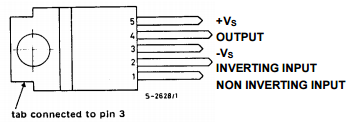
\includegraphics[width=1\textwidth]{img/Print5/TDA2030Pinning.PNG}
	\caption{TDA2030-Pinning}
	\label {fig:3.2.1}
\end{figure}
\subsection{Absolute Maximalwerte}\label{subsec:3.2.1}
Diese Werte wurden zu aller erst mit den Bedingungen an der Schaltung verglichen, da sie ein sehr genaue, kurze Übersicht über den Baustein liefern. (Abb. \ref{fig:3.2.1.1})
\begin{figure} [H]
	\centering
	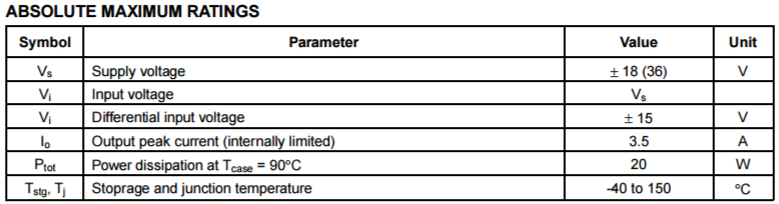
\includegraphics[width=1\textwidth]{img/Print5/TDA2030MaximumRatings.PNG}
	\caption{TDA2030-Pinning}
	\label {fig:3.2.1.1}
\end{figure}

%http://www.itisff.it/dip_eln/tda2030.pdf --> SnippingTool

\section{Filter}\label{sec:3.3}
Es wurde nach einem möglichst steilen, im Durchlassbereich linearen und einfachen Filter gesucht. Man hat sich nach Überlegen für ein \enquote{Aktives-Filter 2.Ordnung} entschieden, dabei wurde die \enquote{Butterworth-Schaltung} bevorzugt. Wegen seiner hohen Linearität im Durchlassbreich und einer Dämpfung von $\frac{-20dB}{Dek.}$ . Dies bedeutet, dass bei einer Tiepfass-Filterung eine Frequenz die 10mal größer ist als die Grenzfrequenz einen um $\frac{1}{10}$ kleineren Pegel aufweist, als die Grenzfrequenz.\\
Zur Regelung wird an den Eingängen (Rechts, Links) und bei der Schaltung (Abb. \ref{fig:5.2.5.1}) auch am Ausgang, jeweils ein Potentiometer in der Größenordnung von 1kOhm verbaut. Diese dienen zur Anpassung der Amplitude des ein- und ausgehenden Signals, um mögliche Übersteuerungen zu vermeiden.

\subsection{Butterworth-Filter 2. Ordnung}\label{subsec:3.3.2}
Die Grundschaltung eines \enquote{Butterworth-Filters 2. Ordnung} ist für verschiedene Grenzfrequenzen die selbe, lediglich die Bauteilwerte variieren. Auch ist die Schaltung der verschiedenen Grundfilterarten unterschiedlich. \\
Die da wären: 
\begin{itemize}
	\item Hochpass
	\item Tiefpass
	\item Bandpass
\end{itemize}
Ein Butterworth-Tiefpass-Filter 2. Ordnung besteht hauptsächlich aus einem OPV, drei Widerständen und zwei Kondensatoren. Deren Anordnung ist ausschlaggebend für das Tiefpass-Filter (Abb. \ref{fig:3.3.2.1}).\\ 
Bedingt durch das Beschalten des OPVs wird das Ausgangssignal invertiert, was hier keine gröberen Folgen mit sich bringt.\\ 
Am Plus-Eingang des OPVs wird entweder Masse bei symmetrischer Spannungsversorgung, oder $\frac{Vcc}{2}$ bei asymmetrischer Spannungsversorgung angelegt.
\begin{figure} [H]
	\centering
	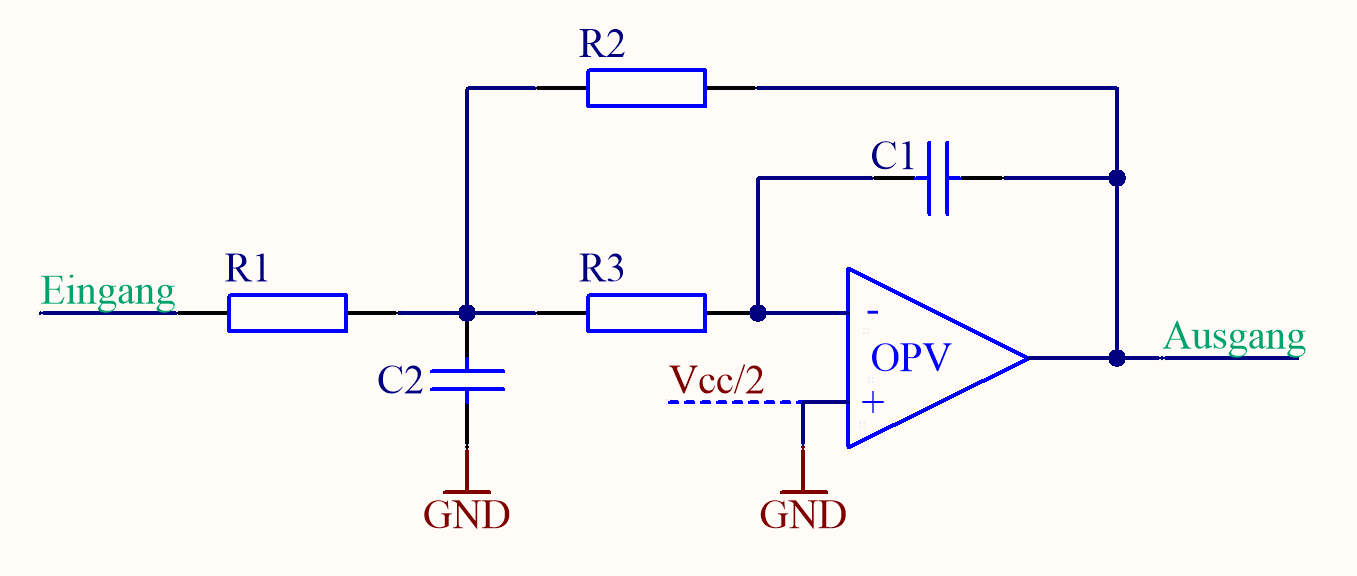
\includegraphics[width=1\textwidth]{img/Print3/TPFilterButterworth2Ordnung.PNG}
	\caption{Butterworth-Tiefpass-Filter 2. Ordnung}
	\label {fig:3.3.2.1}
\end{figure}
Das Bandpass-Filter(\ref{fig:3.3.2.2}) besteht aus drei Widerständen, zwei Kondensatoren und einem OPV, jedoch mit anderer Anordnung als bei dem Tiefpass-Filter.
\begin{figure} [H]
	\centering
	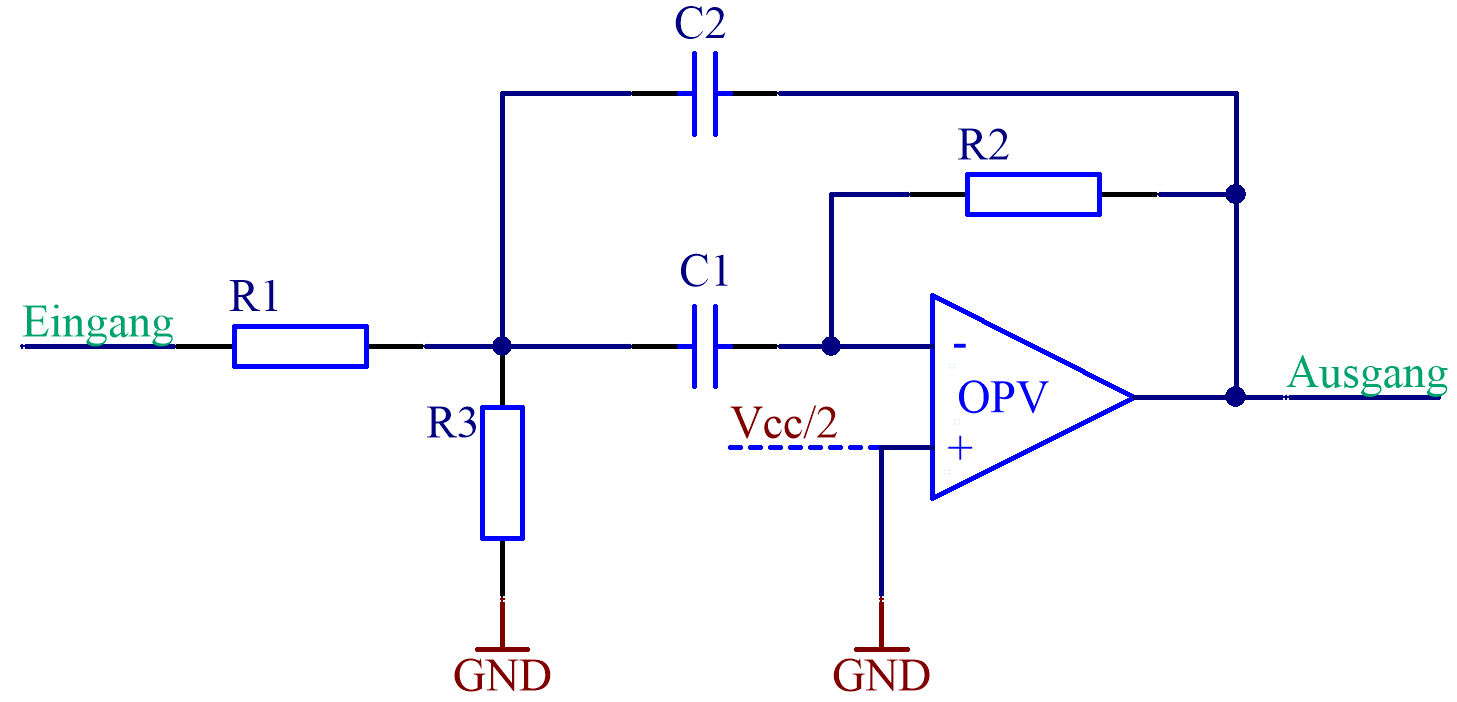
\includegraphics[width=1\textwidth]{img/Print4/BPFilter-Butterworth2Ordnung.PNG}
	\caption{Butterworth-Bandpass-Filter 2. Ordnung}
	\label {fig:3.3.2.2}
\end{figure}
Das Hochpass-Filter(\ref{fig:3.3.2.3}) hat wieder eine ähnliche Konstruktion. Dieses besteht aus drei Kondensatoren, zwei Widerständen und einem OPV. Wiederum in mit bestimmter Anordnung.
\begin{figure} [H]
	\centering	
	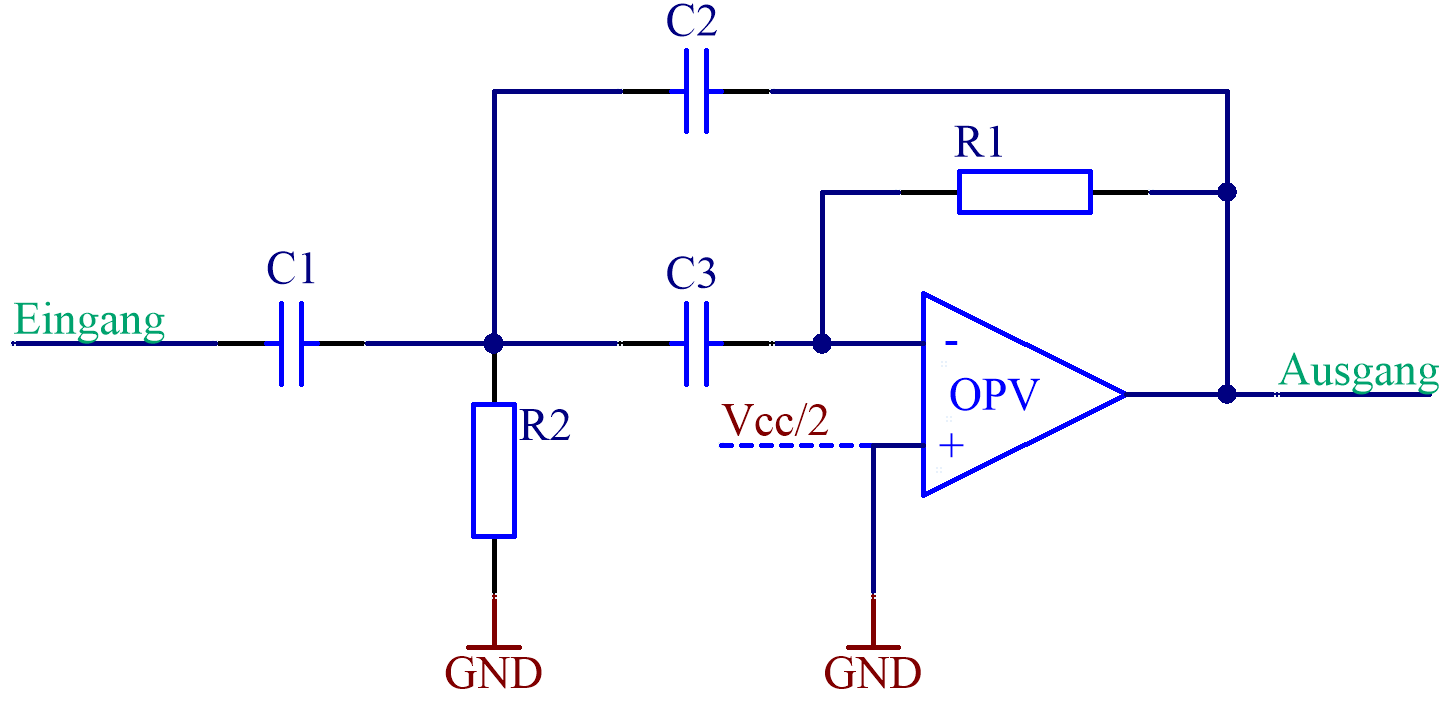
\includegraphics[width=1\textwidth]{img/Print4/HPFilter-Butterworth2Ordnung.PNG}
	\caption{Butterworth-Hochpass-Filter 2. Ordnung}
	\label {fig:3.3.2.3}
\end{figure}

%Selbst generiert in Altium

